\newpage
\section{Embeddings}
\label{sec:embeddings}

A crucial part of the proposed pipeline is to represent the obtained raw telemetry data in a way that abstracts the state of the network, distiniguishing clearly when it is in an anomalous state.
Deep neural networks have been used for non-dynamical graphs \cite{venkatakrishnan_graph2seq_2018}, where the structure of the graph is converted to a continous vector for each timestep.
We need a DNN that can also process the dynamical behavior of our data into the graph.

Another possibility is to use the telemetry data directly, in a fashion similar to Putina et al.\cite{putina_telemetry-based_2018} to feed their clustering algorithm.
However, what is important in our case is that the representations used can distinguished between normal and anomalous network operation.
In order to explore this, we decided to visualize the data and find out if some of the given features could be projected into a lower dimensional space, where a distinction between anomalous and normal behavior is clear.

We started with the data available in the \textbf{telemetry} repository\footnote{https://github.com/cisco-ie/telemetry}, which contains data from experiments with different failure conditions.
The databases contain readings for a subset of the available features for all nodes at different timesteps, pertaining to different Yang paths.
We first constructed a network embedding for each unique timestep, independent of its origin node or Yang path.
Using the ground truth information provided with the datasets, we also tag each timestep as 'anomaly' or 'normal', to use during visualization.
Given the high dimensionality of the resulting vectors, we use the online \textit{Embedding Projector} feature of TensorFlow\footnote{Available at https://projector.tensorflow.org/} to project and visualize them.
Figure \ref{fig:dataset3_all_P100} shows the t-SNE projection from dataset \#3, with blue points representing 'normal' behavior, and red ones timesteps where an 'anomaly' is present.
We notice that this projection does not show a clear division between the two states of interest from this embeddings everywhere.
Instead, it seems that the data can be grouped by the Yang path that produced it, as can be seen in figure \ref{fig:dataset3_all_P100_names}.

\begin{figure}[h!]
	\centering
	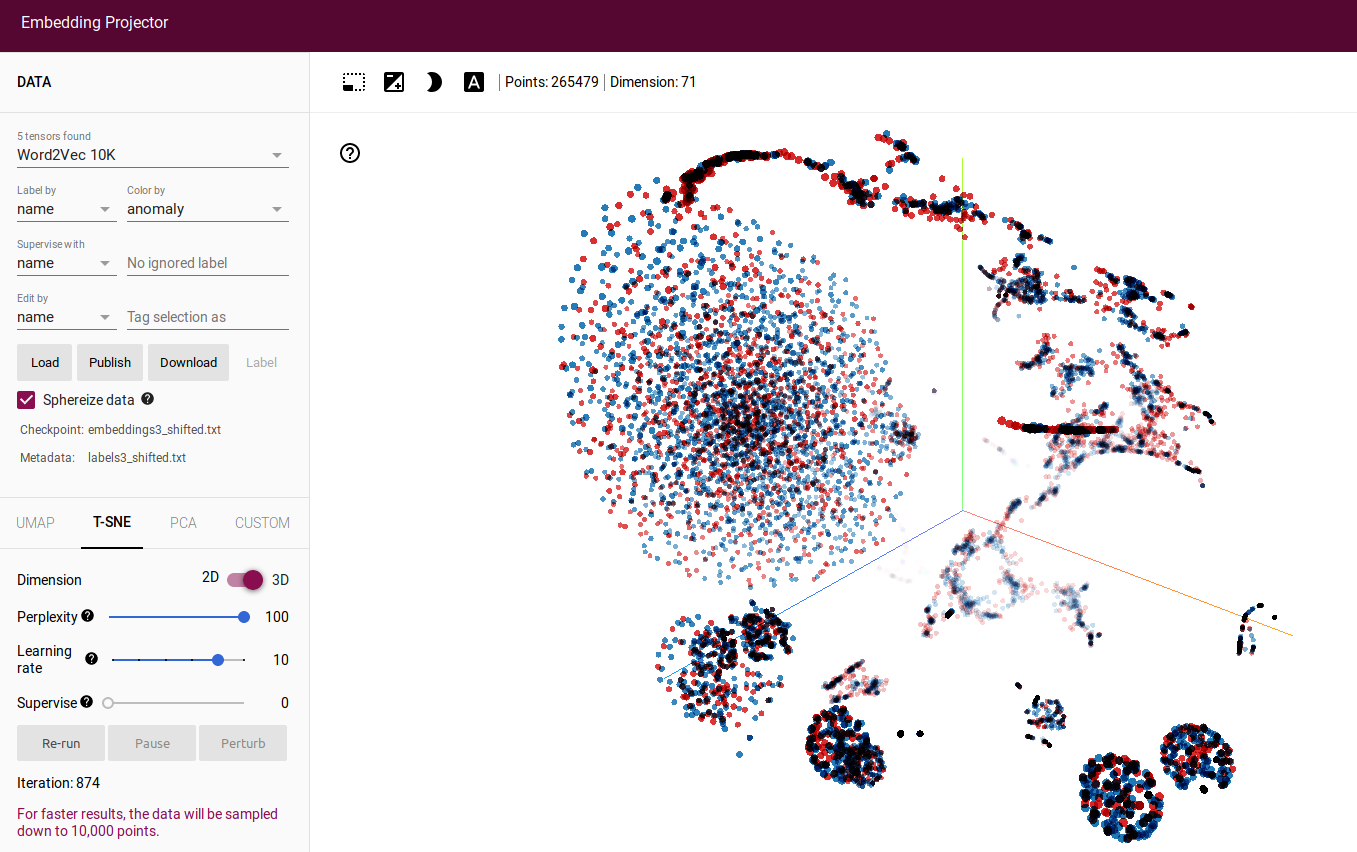
\includegraphics[width=0.8\linewidth]{Figure/dataset3_all_P100.png}
	\caption{t-SNE projection of dataset \#3. Red dots represent timesteps when the system is going through an 'anomaly'.}
	\label{fig:dataset3_all_P100}
\end{figure}
\begin{figure}[h!]
	\centering
	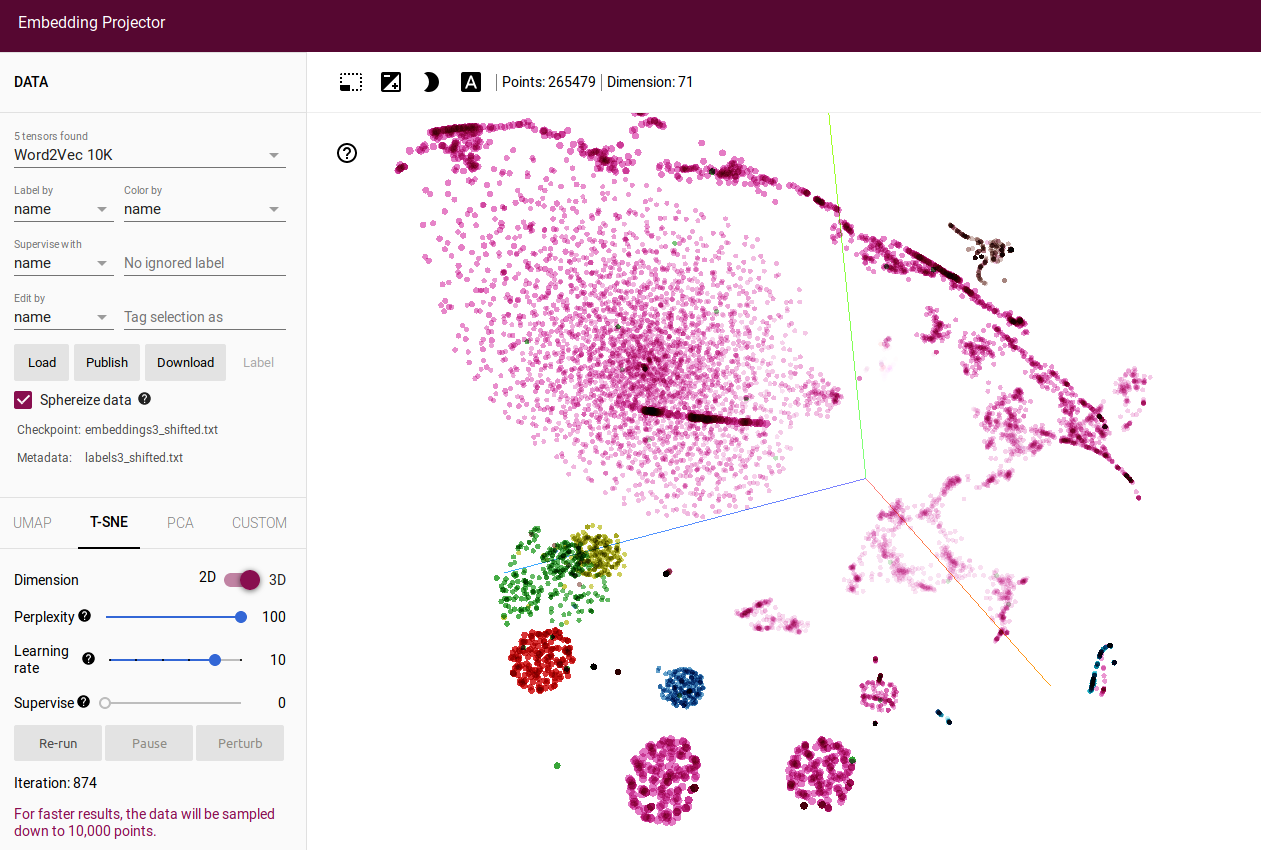
\includegraphics[width=0.8\linewidth]{Figure/dataset3_all_P100_name.png}
	\caption{t-SNE projection of dataset \#3. Color code represents the Yang path that produced each vector.}
	\label{fig:dataset3_all_P100_names}
\end{figure}

Using the \textit{Embedding projector} functionality we are able to isolate the nodes that come from single node, as well as from a specific Yang-path.
We attempt a projection using only the \textbf{leaf1} node, and the \textbf{data-rate} path (the one with most entries), which is shown in figure \ref{fig:dataset3_leaf1_data-rate}.
Although we can see distinction in parts of the data, there are still a big region mixing the two network states of interest.

\begin{figure}[h!]
	\centering
	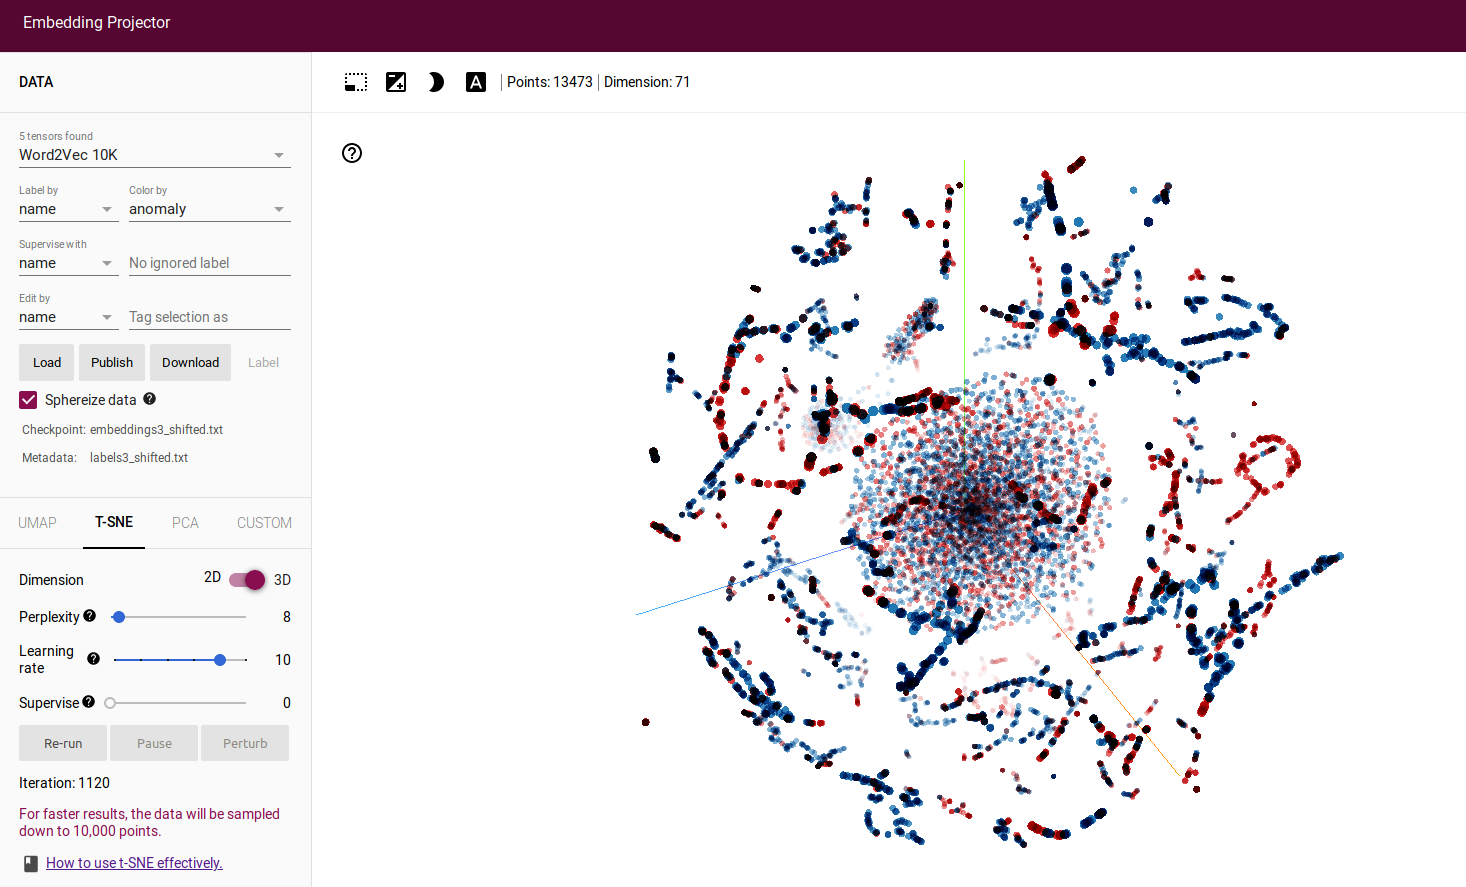
\includegraphics[width=0.8\linewidth]{Figure/dataset3_leaf1_data-rate.png}
	\caption{t-SNE projection of the \textbf{leaf1} node from dataset \#3, using only the features from the \textbf{data-rate} Yang path. The node color distinguish anomalous (red) and normal (blue) states.}
	\label{fig:dataset3_leaf1_data-rate}
\end{figure}

Instead of using pre-selected features, we decide to now project the raw telemetry data available at the \textbf{OutlierDenStream-BigDama18} repository\footnote{https://github.com/anrputina/OutlierDenStream-BigDama18}, which comes separated by node and experiment.
Following Putina et al., we also distinguish between \textit{DataPlane} and \textit{ControlPlane} features to build the node representations for each timestep, discard features which have zero standard deviation, and normalize the resulting data matrix.
Additionaly, the ground truth is used to tag the timesteps where an anomaly is present in the experiment.
The t-SNE projection of node \textbf{leaf1} using the \textit{DataPlane} features is shown in figure \ref{fig:bgpclear_first_leaf1_DP}, where we are able to see a clear distinction between red (anomalous) and blue (normal) network states for this node.

\begin{figure}[h!]
	\centering
	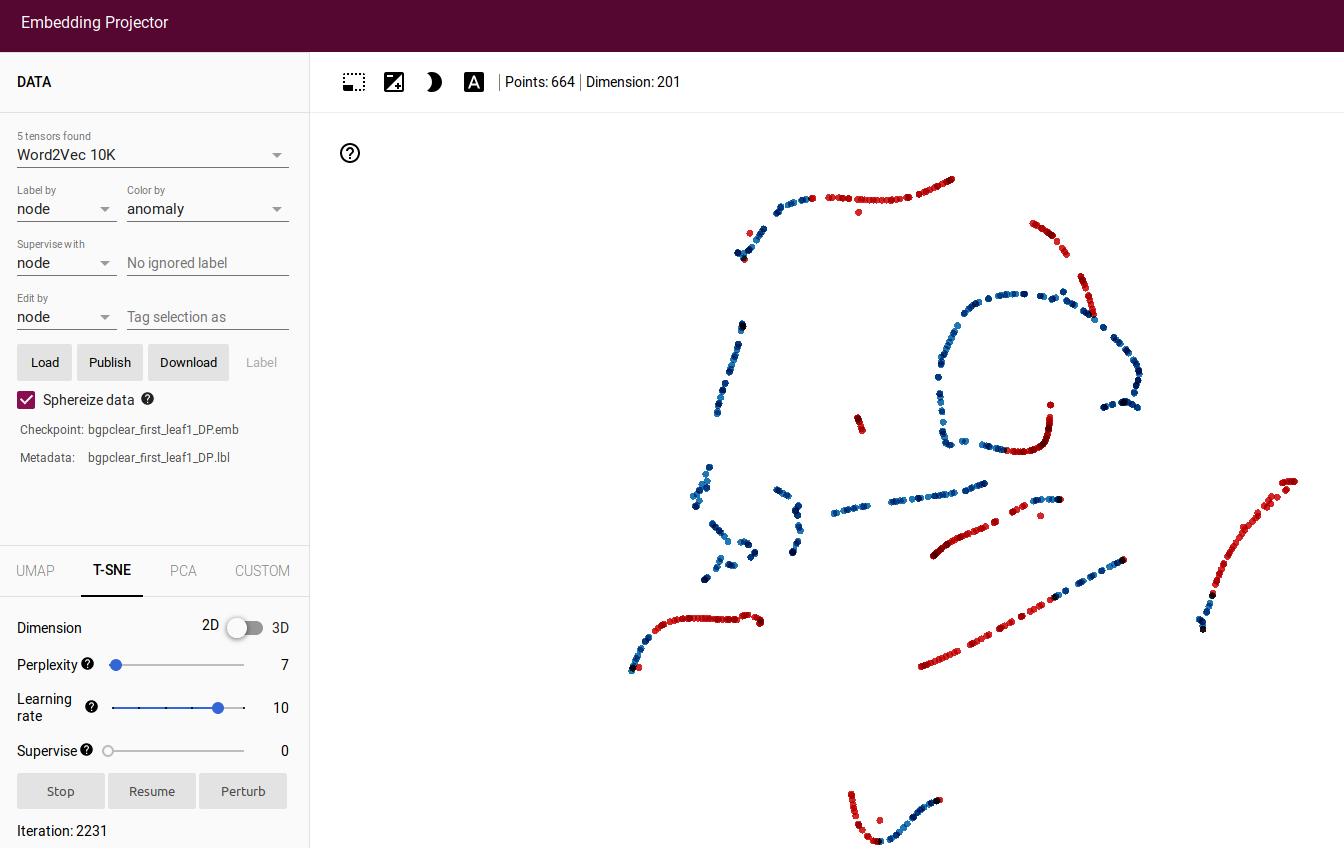
\includegraphics[width=0.8\linewidth]{Figure/bgpclear_first_leaf1_DP.png}
	\caption{t-SNE projection of \textbf{bgpclear\_first}'s \textbf{leaf1} node using \textit{DataPlane} features. Red dots represent timesteps when the system is going through an 'anomaly'}
	\label{fig:bgpclear_first_leaf1_DP}
\end{figure}
\begin{figure}[h!]
	\centering
	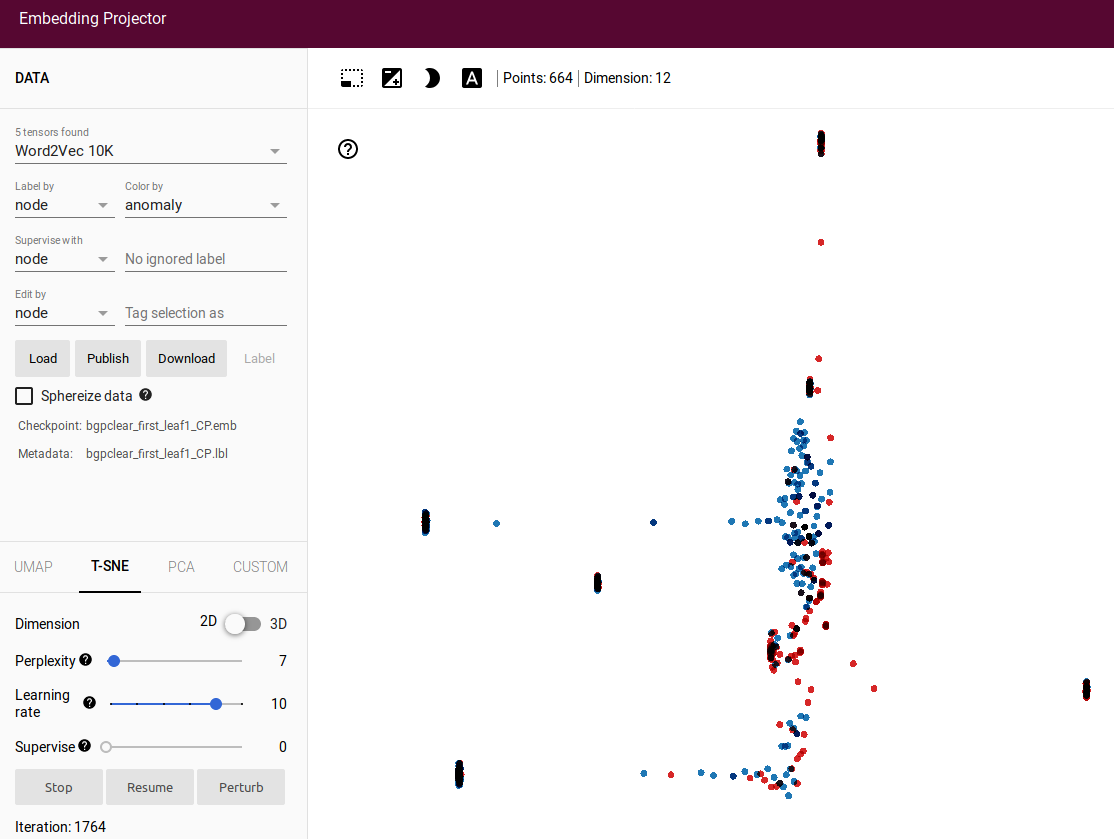
\includegraphics[width=0.8\linewidth]{Figure/bgpclear_first_leaf1_CP.png}
	\caption{t-SNE projection of \textbf{bgpclear\_first}'s \textbf{leaf1} node using \textit{ControlPlane} features. Red dots represent timesteps when the system is going through an 'anomaly'}
	\label{fig:bgpclear_first_leaf1_CP}
\end{figure}

On the other hand, when using the \textit{ControlPlane} for the same node and experiment, we obtain figure \ref{fig:bgpclear_first_leaf1_CP}, which doesn't separate the states of interest as well.

Using data from a different experiment, figure \ref{fig:portflap_first_leaf1_DP} shows that a similar separation of states if found.
\begin{figure}[h!]
	\centering
	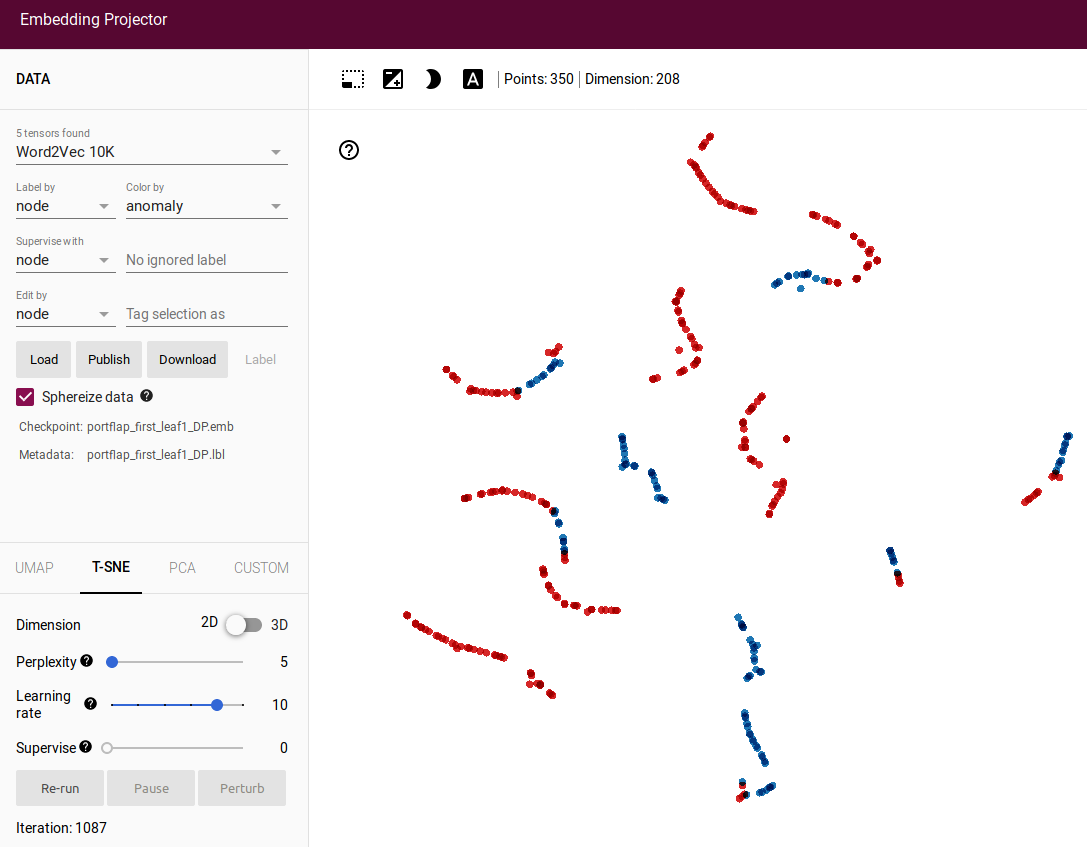
\includegraphics[width=0.8\linewidth]{Figure/portflap_first_leaf1_DP.png}
	\caption{t-SNE projection of \textbf{portflap\_first}'s \textbf{leaf1} node using \textit{DataPlane} features. Red dots represent timesteps when the system is going through an 'anomaly'}
	\label{fig:portflap_first_leaf1_DP}
\end{figure}

This is an interesting result, which shows that it's feasible to subdivide the high-dimensional space in which the given representations exist, and know where the normal behavior of the network lies.
Additionaly, this can be done without having an expert pre-select the features to use, as done by Putina et al\cite{putina_telemetry-based_2018}.
This subdivision of the space will allow to construct the sequence of tokens that would be processed by the Unsupervised Language Learning pipeline to obtain the network's grammar.


